\documentclass[resume]{subfiles}


\begin{document}
\section{Automatiques}
\subsection{Pôles en boucle ouverte}
On calcule les valeurs propres $\lambda$ de $A$
$$\det\left(A-I\lambda\right)=0$$
\subsection{Observateur identité}
Sa dynamique d'erreur est de la forme
$$\dot{\varepsilon}(t)=\dot{z}(t)-\dot{x}(t)=(A-EC)(z(t)-x(t))=(A-EC)\varepsilon(t)$$
Pour déterminer $E$, on utilise la méthode de Ackermann (voir \ref{ackermann}) en remplaçant
$$\begin{cases}
A & \longrightarrow A^{T}\\
B & \longrightarrow C^{T}\\
K & \longrightarrow E
\end{cases}$$
\subsection{Placement de pôles}
Soit un système de la forme
$$\begin{cases}
\dot{x} = Ax+Bu\\
y = Cx + Du
\end{cases}$$
Si l'on souhaite le régler avec un régulateur d'état en utilisant un placement de pôle, on utilise la méthode de Ackermann
\subsubsection{Méthode de Ackermann (exemple avec $n=3$}
\label{ackermann}
On veut utiliser les pôles $p_3,p_2,p_1$. C'est à dire qu'on a un polynôme caractéristique de la forme
$$(s-p_3)(s-p_2)(s-p_1)$$
$$(s-p_3)(s^2-p_2s-p_1s+p_1p_2)$$
$$\textcolor{gray}{a_3}s^3\underbrace{-(p_1+p_2+p_3)}_{a2}s^2+\underbrace{(p_1p_2+p_1p_3+p_2p_3)}_{a1}s\underbrace{-p_1p_2p_3}_{a0}$$
On calcule ensuite la matrice de contrôlabilité
$$M=\begin{pmatrix}
B & AB & A^2B
\end{pmatrix}$$


$$K^T = \begin{pmatrix}
0 & \cdots & 0 & 1
\end{pmatrix}M^{-1}\left(\underset{\underset{1}{\parallel}}{a_3}A^{3}+a_2A^2+a_1A^1+a_0I\right)$$






\subsection{Pôles}
\begin{figure}[H]
\centering
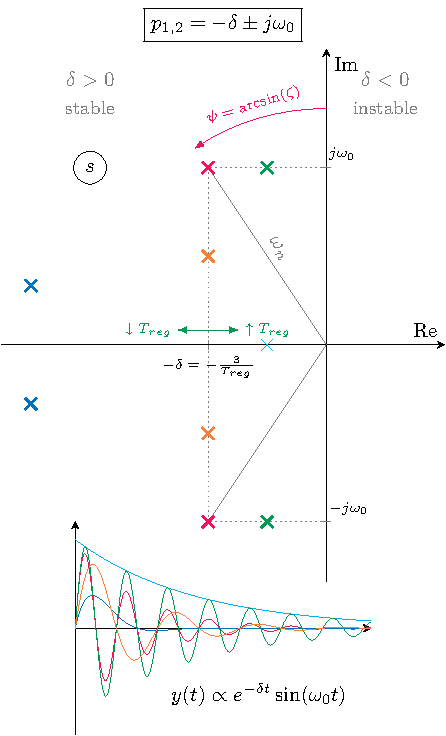
\includegraphics[width=6cm,page=1]{drwg_6.pdf}
\end{figure}

\end{document}